\documentclass[pdf]{beamer}
\mode<presentation>{}
\usepackage{minted}
\usepackage{tikz}
\usepackage{pgffor} %% gives looping with \foreach
\usepackage[absolute,overlay]{textpos}
\usepackage{lmodern} %% scalable latin characters
\usetikzlibrary{arrows,shapes,backgrounds}
\usepackage{multirow}
\usepackage{listings} %% another package for code related stuff


%% stuff for minted
\definecolor{mintedBg}{rgb}{0.95, 0.95, 0.95}
\definecolor{blockBg}{rgb}{0.6, 0.6, 0.95}
\definecolor{rnaColor}{rgb}{0, 0.6, 0}
\definecolor{cdsColor}{rgb}{0, 0.4, 0.4}
\definecolor{rnaPol}{rgb}{0.8,0,0.8}
\definecolor{ribosomeCol}{rgb}{0.5,0.5,0.1}
\definecolor{protColor}{rgb}{0.6,0,0.6}
%% colours for nucleotides:
\definecolor{dACol}{rgb}{0.5, 0.5, 0}
\definecolor{dCCol}{rgb}{0.8, 0, 0}
\definecolor{dGCol}{rgb}{0, 0.8, 0}
\definecolor{dTCol}{rgb}{0, 0, 0.8}

\definecolor{navy}{rgb}{0, 0, 0.6}
\definecolor{pur}{rgb}{0, 0, 0.6}
\definecolor{pyr}{rgb}{0.6, 0, 0.2}
%% define styles for different codes
\newminted{cpp}{linenos, bgcolor=mintedBg, fontsize=\footnotesize}
%% then use \begin{cppcode}
\newminted{c}{linenos, bgcolor=mintedBg, fontsize=\footnotesize}
\newminted{perl}{linenos, bgcolor=mintedBg, fontsize=\footnotesize}
\newminted{sh}{linenos, bgcolor=mintedBg, fontsize=\footnotesize,
  language=bash}
\newminted{console}{linenos, bgcolor=mintedBg, fontsize=\footnotesize}

%% a command to define a subheading
\newcommand\subHeading[1]{
  \par\bigskip {\Large\bfseries#1}\par\smallskip
}

%% I detest indentation in footnotes etc, so try this:
\makeatletter
\renewcommand\@makefntext[1]{\noindent\makebox[0em][r]{\@makefnmark}\tiny#1}
\makeatother
%% the makeatletter and makeatother are required to allow me to
%% to change the macro beginning with an @. (though when I call it
%% I don't use the @ ... 

\setlength\parskip{0.5em}
\setlength\parindent{0ex}

%% to have footnotes without references. This from tex.stackexchange.com
\newcommand\blfootnote[1]{%
  \begingroup  %% this makes it a local redefinition
  \renewcommand\thefootnote{}\footnote{#1}%
  \addtocounter{footnote}{-1}  % this adjusts the footnote counter
  \endgroup
}


\title{A brief introduction to perl}
\subtitle{Doing something useful in perl}
\author{Martin Jakt}

\begin{document}

\begin{frame}
  \titlepage
\end{frame}

\begin{frame}[fragile]{perl}
  possibly:

  Practical Extraction and Reporting Language

  but this is not offical. Perl / perl, I've got no idea but have seen
  opinions as to this expressed on the web.
\end{frame}

\begin{frame}[fragile]{why perl}
  \begin{enumerate}
  \item It's easy to learn enough to do something useful.
  \item Quite a lot of genomics tools still use perl.
  \item Used to be the biggest language in bioinformatics.
  \item Good for text handling; making it useful for file munging (converting
    formats).
  \end{enumerate}
\end{frame}

\begin{frame}[fragile]{why not perl}
  \begin{enumerate}
  \item Kind of old and decrepit compared to the new bunch of languages.
  \item Rather slow for mathematical stuff.
  \item New projects more likely to use something like Python or R.
  \item Yeah, the code is kind of ugly...
  \end{enumerate}

  but we don't care, as it demonstrates how to string together simple
  actions to make something big.
\end{frame}


\begin{frame}[fragile]{topics covered}
  \begin{enumerate}
  \item Installing perl (only for Windows)
  \item Running a script
  \item Simple variable types
  \item Less simple variable types
  \item Accessing the script arguments
  \item Opening files for reading and writing
  \item Parsing text with regular expressions
  \item Making functions (subroutines)
  \item Doing something useful with all of this.
  \end{enumerate}
\end{frame}

\begin{frame}{Warnings}
  \begin{itemize}
  \item I am not a perl expert.
  \item I learnt perl a long time ago. Some things have moved on.
  \item I've only ever bothered to learn enough to solve my problems.
  \end{itemize}

  But programming is about building big things from small components; so don't
  care too much!
    
\end{frame}

\begin{frame}{perl on Windows}
  \url{http://padre.perlide.org/}
  \begin{figure}[ht]
    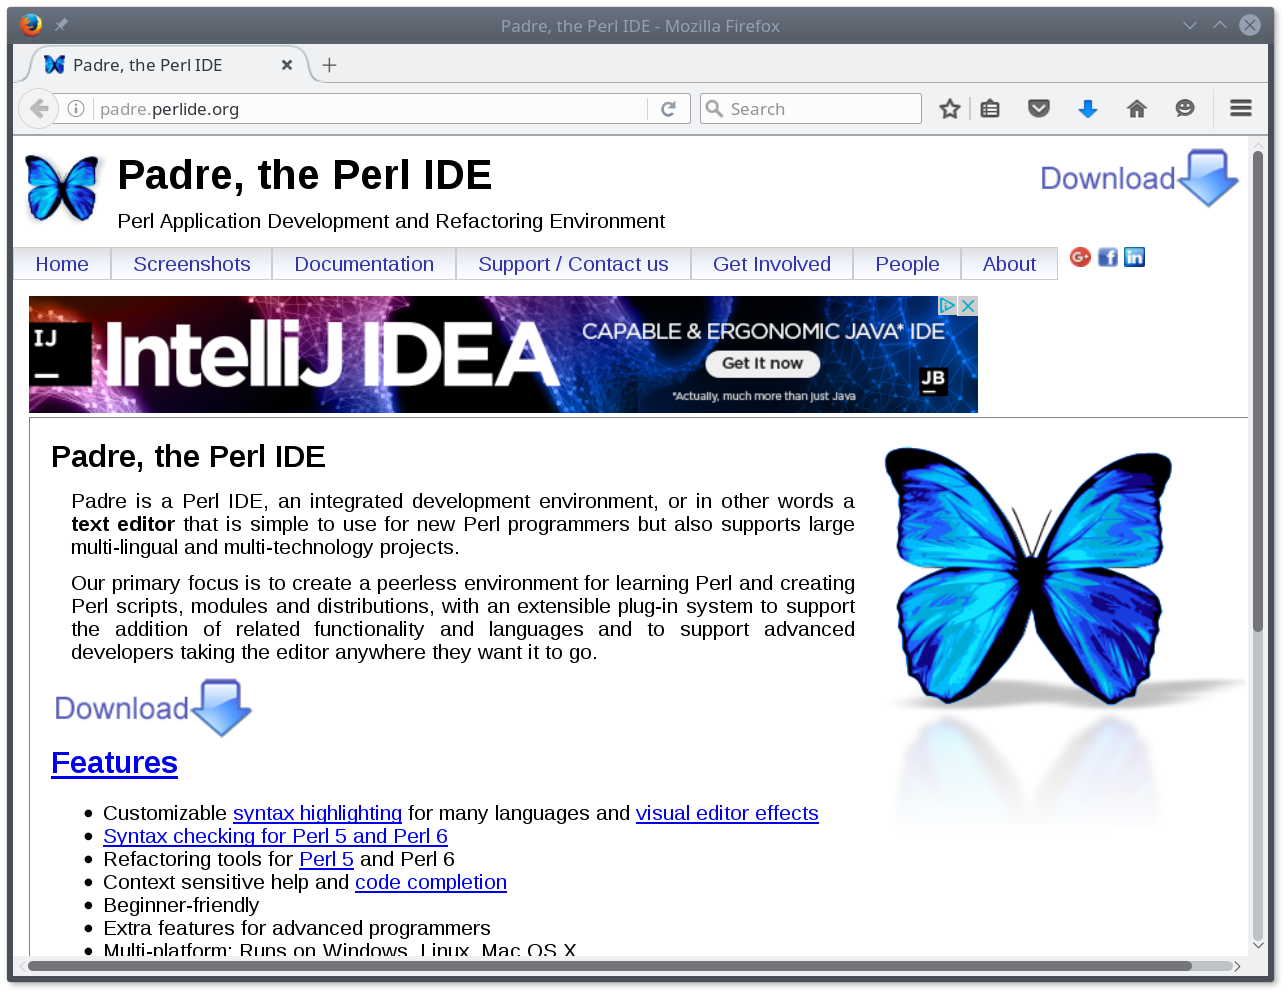
\includegraphics[width=0.8\textwidth]{images/padre_website.png}
  \end{figure}
  follow the links to the download page. Get the DWIM Perl.
\end{frame}

\begin{frame}{a decent console for windows}
  \url{https://github.com/cbucher/console/wiki/Downloads}
  \begin{figure}[ht]
    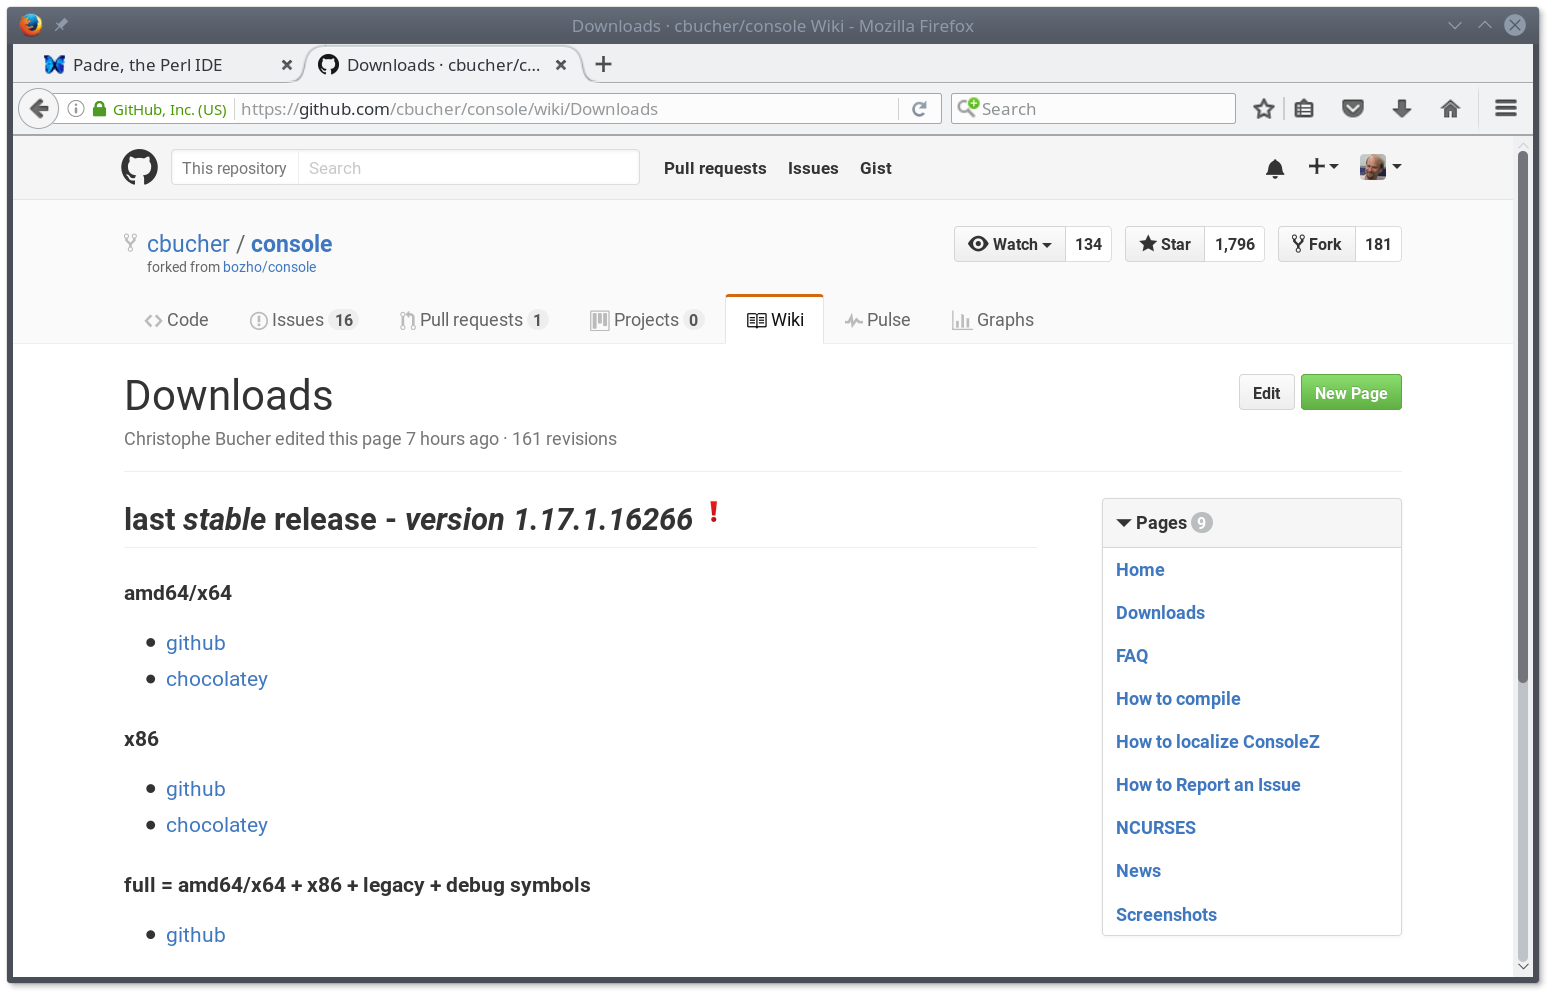
\includegraphics[width=0.8\textwidth]{images/consolez_website.png}
  \end{figure}
  Again, follow the download links.
\end{frame}

\begin{frame}{a text editor for the mac?}
  not sure: you can try textmate at:\\
  \url{http://macromates.com/download}\\

  or have a look at the options at:\\
  \url{http://beebom.com/best-text-editors-for-mac/}
\end{frame}

\begin{frame}{online tutorials}
  There are lots of online perl tutorials.

  if you are too lazy to google, you can go to:

  http://perlmaven.com/perl-tutorial

\end{frame}

\begin{frame}[fragile]{a first program}
  Open your editor or IDE (Padre) and enter the following:

  \begin{perlcode}
    print "Hello world\n";
    for $w(@ARGV){
      print $w, "\n";
    }
  \end{perlcode}

  Save this file at a suitable location. Then open a console: on Windows you
  can use 'ConsoleZ.exe' or 'cmd.exe'. On Macs open a terminal. Navigate to
  the directory where you saved the above perl script (eg. hello.pl) and type:

  \begin{consolecode}
    perl hello.pl one two three four
  \end{consolecode}

  and see what happens.
\end{frame}

\begin{frame}[fragile]{the \#! in unix}
  You will usually see something like:
 
  \begin{perlcode}
    #!/usr/bin/perl -w
  \end{perlcode}

  at the beginning of most perl scripts. This is useful on Unix based systems
  (probably Macs as well, but it may need to be modified), but does nothing on
  Windows systems.

  On Unix systems, it allows the script to be run without explicitly invoking
  the perl interpreter, as this is taken care of by the shell.
\end{frame}

\begin{frame}[fragile]{warnings!}
  On Unix systems:
  
  \begin{perlcode}
    #!/usr/bin/perl -w
  \end{perlcode}

  causes the perl interpreter to be run on the source code. The \texttt{-w}
  option causes the interpreter to issue warnings when it comes across strange
  or incorrect things. You should always use this; but if you run the script
  with:

  \begin{consolecode}
    perl script_name.pl
  \end{consolecode}
 
  this won't help.

\end{frame}

\begin{frame}[fragile]{warnings and other decrees}
  To ensure warnings are used you can do:
  
  \begin{consolecode}
    perl -w script_name.pl
  \end{consolecode}

  but the script writer might wish to enforce use of warnings. In this case
  it's better to use:
  
  \begin{perlcode}
    #!/usr/bin/perl
    use warnings;
  \end{perlcode}
  
  at the beginning of the file. This way warnings will be used regardless of
  how the script is run.
\end{frame}

\begin{frame}[fragile]{strict!}
  If you have a look some perl tutorials they will suggest strongly:

  \begin{perlcode}
    #!/usr/bin/perl
    use warnings;
    use strict;
  \end{perlcode}
  
  The \texttt{use strict} effectively changes perl's core behaviour regarding
  scope. It forces you to declare variables such that their scope is defined.

  This is good, and probably essential for any larger perl project. You should
  probably \texttt{use strict;} in your code. But I don't normally bother as I
  will use a different language for anything more complex.
\end{frame}

\begin{frame}[fragile]{strict!}
  an example:
  \begin{perlcode}
    #!/usr/bin/perl
    use warnings;
    use strict;
    
    ## here the scope of $a is anyway global
    ## so my doesn't do anything.
    my $a = 10;

    for my $i(0..10){
      ## this is not allowed
      $c = $a * $i;
      ## but this is:
      my $d = $a * $i;
    }
    \end{perlcode}
\end{frame}


\begin{frame}[fragile]{Variable types}
  \small{
  \begin{itemize}
  \item \textcolor{navy}{Scalars} hold single values and dare enoted by the \texttt{\$} prefix.
    \begin{perlcode}
  $a = 10;
  $b = "hello world"
    \end{perlcode}
  \item \textcolor{navy}{Arrays} hold a series of values and are denoted by the \texttt{@}
    prefix. Individual values are accessed by their index as
    scalars (i.e. using a \texttt{\$} prefix).
    \begin{perlcode}
  @array = (1, 2, 3, 4);
  $array[0] = 10;
  ## the array now holds values 10, 2, 3, 4
    \end{perlcode}
  \item \textcolor{navy}{Hashes} hold key-value pairs and are denoted by the \texttt{\%}
    prefix. Individual values are accessed using the key value in curly
    brackets.
    \begin{perlcode}
  %fruit_colors = (apple => 'green', orange => 'orange');
  print "an apple is ", $fruit_colors{apple}, "\n";
  ## will print 'an apple is green'
    \end{perlcode}
  \end{itemize}
}
\end{frame}


\begin{frame}[fragile]{Data types}
  In computing there are in essence three types of data:
  \small{
   \begin{itemize}
   \item \textcolor{navy}{text} This is simply strings of bytes that do not
     have any implicit meaning or encoding. In bioinformatics text is usually
     encoded using ASCII, but this can change.
   \item \textcolor{navy}{integers} These hold integral values using a fixed
     number of bytes per integer. The number of
     different integrals that can be encoded depends on the number of bytes
     used.
   \item \textcolor{navy}{floats} These hold an approximation of real numbers,
     encoded using an exponential form giving variable precision.
   \end{itemize}

  perl is dynamically typed. That means perl tries to guess what the
  appropriate data type should be, printing warnings or giving up when asked
  to do something stupid.
}
  \begin{perlcode}
    $a = 1;
    $b = "two";
    print "1 + two = ", $a + $b, "\n";
    ## this will print a warning message.
  \end{perlcode}

\end{frame}

\begin{frame}[fragile]{Text data}
  Text is complicated. But perl normally handles text pretty well. For now
  you can think of text as being the characters that you enter using the
  keyboard.

  Plus some non-printable characters like newlines (when you press return),
  tabs and carriage returns (?).

  In perl, just be aware of the difference between \texttt{"} and \texttt{'}.

  \begin{perlcode}
    $word = "hello";
    $word2 = 'world';
    $sentence1 = "$word1 $word2";
    $sentence1 = '$word1 $word2';
  \end{perlcode}
\end{frame}

\begin{frame}[fragile]{Single and double quotes}
  The code:
  \begin{perlcode}
  $word1 = "hello";
  $word2 = 'world';
  $sentence1 = "$word1 $word2";
  $sentence1 = '$word1 $word2';

  print "$sentence1\n";
  print "$sentence2\n";
  \end{perlcode}
  
  will print:
  \begin{consolecode}
  hello world
  $word1 $word2
  \end{consolecode}

  Can you work out what's going on?
\end{frame}

\begin{frame}[fragile]{Double quotes and printing}
  The use of \texttt{"} causes perl to look into the quoted string and
  replacing strings that look like variables with their values.

  This means this works:
  \begin{perlcode}
    $word = 'hello';
    print "the word is $word\n";
  \end{perlcode}

  I sometimes prefer to give variables to print statements as separate
  arguments:
  \begin{perlcode}
    print "the word is ", $word, "\n";
  \end{perlcode}

  as it makes it easier to see the use of the variable when using syntax highlighting.
\end{frame}

\begin{frame}[fragile]{Arrays}
  \small As indicated above we can initiate an array with a set of values using a
  comma seperated list:

  \begin{perlcode}
    @x = (1, 10, 100, 1000);
  \end{perlcode}

  \small If we want to make an array of text elements we need to quote them:
  \begin{perlcode}
    @s  = ('one', 'two', 'three');
  \end{perlcode}

  \small But most frequently we do not do this, as the arrays normally hold data
  which we will obtain from some file somewhere. In this case we may:

  \begin{perlcode}
    $x[0] = 1;
    $x[1] = 10;
    $s[2] = 100;
  \end{perlcode}

  \small Note that the indexing starts from 0, not 1, and that both the index and the
  value would normally be generated by the program logic (not written in the
  code directly!).
  
\end{frame}

\begin{frame}[fragile]{Looping through arrays}
  The array holds a set of values. We can get the length of an array in two
  different ways:
  
  \begin{perlcode}
    @ar1 = (1, 2, 3);
    print 'The length of @ar1 is ', scalar( @ar1 ), "\n";
    print 'The highest index of @ar1 can be accessed ',
           'using $#ar1 and is: ', $#ar1, "\n";
  \end{perlcode}

  We can use this information to go through each element of an array and do
  something useful.
\end{frame}

\begin{frame}[fragile]{Looping through arrays (1)}
  The classic loop:
  \begin{perlcode}
  @x = (1, 10, 100, 1000);
  for( $i=0; $i < @x; $i++){
    $l[$i] = log($x[$i]) / log(10);
  }
  \end{perlcode}
  \small{
  This loop starts with three part statement seperated by semicolons.
  \begin{itemize}
  \item The initial state: sets some starting condition; here we set the value
    of \verb|$i| to 0. We will use \verb|$i| as an index to access individual
    elements.
  \item A condition which must be true for the loop to enter
    step. Here we use \verb|$i < @x|. Here \verb|@x| is evaluated as a scalar
    value and enumerates to the length of the array. So we will continue as
    long as \verb|$i| is less than the length of the array.
  \item An action to be carried out at the end of each step before the
    conditional is evaluated. Here we simply say \verb|$i++|, which will
    increment the value of \verb|$i| by 1. If we used, \verb|$i += 2|, then we
    would only look at evenly indexed elements of the array.
  \end{itemize}
}
\end{frame}

\begin{frame}[fragile]{Looping through arrays (2)}
  We can also use a \texttt{while} loop to simulate the classic loop:
  
  \begin{perlcode}
  @x = (1, 10, 100, 1000);
  $i = 0;
  while($i < @x){
    $l[$i] = log($x[$i]) / log(10);
    $i++;  ## don't forget this!
  }
  \end{perlcode}

  If you forget to increment \verb|$i| you will end up with an infinite
  loop. Use \texttt{Ctl-C} to stop this.
\end{frame}


\begin{frame}[fragile]{Looping through arrays (3)}
  Using a range notation

  \begin{perlcode}
  @x = (1, 10, 100, 1000);
  for $i(0..$#x){
    $l[$i] = log($x[$i]) / log(10);
  }
  \end{perlcode}
  
  This simply says: set the value of \verb|$i| to each value in the range of 0 to the highest index
  (i.e. the length - 1) of \verb|@x| and do the stuff within the next bit of
  code (enclosed by the curly brackets).
\end{frame}


\begin{frame}[fragile]{Looping through arrays (4)}
  Getting the values by perl magic:
  
  \begin{perlcode}
  @l = (); ## ?? what are we doing here?? 
  @x = (1, 10, 100, 1000);
  for $v(@x){
    push @l, log($v) / log(10);
  }
  \end{perlcode}
  
  This simply says: assign each value of \verb|@x| (one at a time) to
  \verb|$v| and do the stuff in the loop body (the following block of code).

  Since we do not get an index value here we can not create the \verb|@l|
  array like we did in the previous loops. Instead we create an empty array
  and use \verb|push| to add elements to its end.
\end{frame}

\begin{frame}[fragile]{push, pop, shift and unshift}
  perl has a set of functions that let you add or remove elements to the ends
  of arrays:
  \begin{description}
    \item[push] Adds an element to the end of an array.
    \item[pop] Removes an element from the end of an array and returns it.
    \item[shift] Removes an element from the front of an array and returns it.
    \item[unshift] Adds an element to the beginning of an array.
  \end{description}

  We can use pop and shift to loop through the elements of an array whilst
  also emptying the array.
\end{frame}

\begin{frame}[fragile]{looping and emptying an array}
  Use \texttt{shift} to empty the array from the first to the last element:
  \begin{perlcode}
  @x = (1, 10, 100, 10000);
  @l = ();
  while( $v = shift(@x) ){
    push @l, log($v) / log(10);
  }
  \end{perlcode}
  
  Use \texttt{pop} to reverse the order:
  \begin{perlcode}
  @x = (1, 10, 100, 1000);
  @l = ();
  while( $v = pop(@x) ){
    push @l, log($v) / log(10);
  }
  \end{perlcode}

  What does that result in?
\end{frame}

\begin{frame}[fragile]{negative indices}
  \begin{perlcode}
  @x = (1, 10, 100, 1000);
  print "-1 : ", $x[-1], "\n";
  print "-2 : ", $x[-2], "\n";
  \end{perlcode}
  
  \hspace{1cm} $\Downarrow$

  \begin{consolecode}
  -1 : 1000
  -2 : 100
  \end{consolecode}
  
  Negative indices simply count from the end of the array.
\end{frame}

\begin{frame}[fragile]{2 and n-dimensional arrays}
  perl doesn't have any native matrix class as such, but these can be
  simulated with arrays of arrays:

  \begin{perlcode}
  $width = 10;
  $height = 5;
  @table = ();
  for($y=0; $y < $height; $y++){
    for($x=0; $x < $width; $x++){
      $table[$y][$x] = 0;
    }
  }
  \end{perlcode}

  This basically works... But there are some complications for accessing the
  sizes of the lower order arrays.
\end{frame}

\begin{frame}[fragile]{True and False values?}
  True and False are also known as boolean values.
  
  Consider the following operation:
  \begin{perlcode}
    10 < 1;
  \end{perlcode}

  The statement is clearly False, and the operation returns a \texttt{FALSE}
  boolean value. This can be used in conditionals (if, while, etc...).

  Consider also:
  \begin{perlcode}
    while( $v = shift @x ){  do_stuff($v); }
  \end{perlcode}
  
  Here the assignment to \verb|$v| can fail if the array is empty. When this
  happens the assignment operation itself returns a \texttt{FALSE} value, and
  the loop body is not entered.

  In general any non-0 value is considered true; only 0 is special. However,
  there is likely to be some magic in perl to complicate things.
\end{frame}

\begin{frame}[fragile]{Hashes}
  These store key-value pairs, are prefixed with \verb|%| and accessed as
  scalars using curly brackets \verb|{}|

  \begin{perlcode}
  %capitals = (japan => 'Tokyo',
               UK => 'London',
               norway => 'Oslo');

  print "The capital of Norway is $capitals{norway}\n";

  ## add a new entry to the hash
  $capitals{france} = 'Paris';
  \end{perlcode}

  \begin{itemize}
  \item You don't have to use quotation marks when specifying the key.
  \item Note the multiline statement terminated by ;
  \end{itemize}
  
\end{frame}

\begin{frame}[fragile]{traversing hashes}
  To traverse a hash first get the keys using the \texttt{keys} function:

  \begin{perlcode}
  ## %capitals was already defined somewhere else
  @countries = keys %capitals;
  for $country(@countries){
    print "capital of $country is : $capitals{$country}\n";
  }
  \end{perlcode}
\end{frame}

\begin{frame}[fragile]{A hash of arrays}
  To make a hash of arrays one can simply do:
  
  \begin{perlcode}
  for $i(0..10){
    $g_exp{gene1}[$i] = $i;
    $g_exp{gene2}[$i] = $i * 2;
  }
  \end{perlcode}

  Accessing elements of this is a bit more painful.
\end{frame}

\begin{frame}[fragile]{complex data structures}
  When we make an array of arrays, or an array of hashes, what we actually
  make is an array of references to arrays or hashes. You can see this by this
  bit of code;

  \begin{perlcode}
    for $x(0..2){
      for $y(0..2){
        $ar[$x][$y] = 0;
      }
      print "ar[$x] : $ar[$x]\n";
    }
  \end{perlcode}
  
  which will print:
  \begin{consolecode}
    ar[0] : ARRAY(0x132b1c0)
    ar[1] : ARRAY(0x132b118)
    ar[2] : ARRAY(0x132b0d0)
  \end{consolecode}

  So how can we access the elements if we do not know the dimensions?
\end{frame}

\begin{frame}[fragile]{dereferencing intermediates (1)}
  Complex data structures are implemented with references. To traverse them we
  need to be able to de-reference intermediate elements.
  \begin{perlcode}
  for $x(0..2){
    for $y(0..2){
      $ar[$x][$y] = 0;
    }
  }
  \end{perlcode}
  
  \small If we want to know the length of the  array pointed to by \verb|$ar[$i]| we
  cannot simply do \verb|$#ar[$i]| because \verb|$ar[$i]| is just a scalar
  variable that points or references an array. To dereference it we use more
  curly brackets. To get the highest index: \verb|$#{$ar[$i]}|, to get the
  actual array \verb|@{$ar[$i]}|.
\end{frame}

\begin{frame}[fragile]{dereferencing intermediates (2)}
  Curly brackets to the rescue:
  \begin{perlcode}
  for $x(0..2){
    for $y(0..2){
      $ar[$x][$y] = 0;
    }
  }
  ## to go through this we can do:
  for $x(0..$#ar){
    for $y(0..$#{$ar[$x]}){
      $ar[$x][$y] = 1;
    }
    ## or we can use the classic way
    for($y=0; $y < @{$ar[$x]}; $y++){
      $ar[$x][$y] = 2;
    }
  }
  \end{perlcode}
  which is pretty ugly...
\end{frame}

\begin{frame}[fragile]{dereferencing intermediates (3)}
  For a hash of arrays...
  \begin{perlcode}
  for $i(0..1){
    $hash{el1}[$i] = $i;
    $hash{el2}[$i] = $i * 2;
  }
  
  @keys = keys %hash;
  for $k(@keys){
    for $i(0..$#{$hash{$k}}){
      print "$k\t$i\t$hash{$k}[$i]\n";
    }
  }
  \end{perlcode}

  results in:
  \begin{consolecode}
  el1     0       0
  el1     1       1
  el2     0       0
  el2     1       2
  \end{consolecode}
\end{frame}

\begin{frame}[fragile]{Another way to make arrays of arrays}
  \begin{perlcode}
  @ar1 = (2, 4, 8);
  @ar2 = (10, 100, 100); 
  $ar3[0] = [ @ar ];
  $ar3[1] = [ @ar ];

  print "i  j  value\n";
  for $i(0..$#ar3){
    for $j(0..$#{$ar3[$i]}){
      print "$i  $j  $ar3[$i][$j]\n";
    }
  }
  \end{perlcode}

  \hspace{1cm} $\Downarrow$

  \begin{consolecode}
  i  j  value
  0  0  2
  0  1  4
  0  2  8
  1  0  10
  1  1  100
  1  2  1000
  \end{consolecode}

\end{frame}

\begin{frame}[fragile]{Enough about data structures!}
  Accessing the script arguments/

  These are present in the \verb|@ARGV| array. You can access them like any
  array, as shown above.

  \begin{perlcode}
  #!/usr/bin/perl -w
  ## this simply echoes all of the argument variables.
  while( $a = shift @ARGV ){
    print $a, "\n";
  }
  \end{perlcode}
  
  \hspace{1cm} $\Downarrow$

  \begin{consolecode}
  > ./echo.pl hello world
  hello
  world
  \end{consolecode}

\end{frame}

\begin{frame}[fragile]{Opening a file for reading or writing}
  Files are opened with the \texttt{open()} command. There are some variants,
  but common usage is:

  \begin{perlcode}
  $fileName = $ARGV[0];
  ## to open for reading:
  open($fh1, "<", $fileName) || 
       die "unable to open $fileName $!\n";
  
  ## to open for writing:
  open($fh1, ">", $fileName) || 
       die "unable to open $fileName $!\n";

  ## to open for appending:
  open($fh1, ">>", $fileName) || 
       die "unable to open $fileName $!\n";
  \end{perlcode}

  \small The \verb|$fh1| variable is a filehandle that is used to read or write data
  from the opened files. The \verb#|| die "unable to open $filename $!# is
  used to make sure that the file opened.

\end{frame}

\begin{frame}[fragile]{Reading data}
  open the file:
  \begin{perlcode}
  open($fh1, "<", $fileName) || 
       die "unable to open $fileName $!\n";
  \end{perlcode}

  \small Here \verb#||# is symbolic for 'or'. The meaning is, open the file or
  die. If the open command fails the script will terminate with an error
  message that includes the value of \verb|$!| variable. This is the internal
  error string. In fact you can write 'or' instead of \verb#||#, but it's good
  to know both.

  Read the file line by line using a loop:
  \begin{perlcode}
  while(<$fh>){
    print;
    chomp;
    ## do something with the line
  }
  \end{perlcode}
  ??? \texttt{print}, \texttt{chomp}, functions called with no arguments ??
\end{frame}

\begin{frame}[fragile]{the default variable}
  To read a line of text from a file we use the \verb|<$fh>| operator. This
  returns one line of text; if you don't specify a variable
  (eg. \verb|$l = <$fh>|) the line will be assigned to the \verb|$_| variable.
  
  This is the default variable; if you call functions without any arguments perl
  will often (always?) try this one.
  
  \texttt{chomp} is a function that removes a trailing newline (\verb#\n#) if
  it exists. If no argument is given it will remove the line 

\end{frame}


\begin{frame}[fragile]{printing to file}
  Open the file you wish to print to:
  \begin{perlcode}
  $fn = shift @ARGV; ## takes the first argument in @ARGV
  open($fh, ">", $fn) or die "unable to open $fn $!\n";
  print $fh "This text will go to the into the specified file\n";
  \end{perlcode}
  
  simple, but not terribly useful if simply like this.

\end{frame}

\begin{frame}[fragile]{handling text}
  functions and operators for text:
  \begin{description}
  \item[\texttt{.}] The concatenate operator. This returns the concatenation
    of its operands.
  \item[\texttt{.=}] This concatenates the right operand to the left operand.
  \item[\texttt{\textasciitilde=}] The regular expression operator. This looks for matches in
    its left operand to the pattern specified in its right operand. It returns
    \texttt{TRUE} if the pattern is found.
  \item[\texttt{substr}] lets you extract substrings from strings.
  \item[\texttt{split}] splits strings on matches to a regular expression;
    returns an array of the resulting substrings.
  \end{description}

  \small  Regular expressions is a complicated topic, and will only be introduced very
  briefly here. See Perl\_intro.pdf for more details, use google to read more
  and experiment with code to learn.

\end{frame}

\begin{frame}[fragile]{comparing texts}
  In perl different comparison operators are used for strings and numbers:
  \begin{description}
  \item[\texttt{==}] tests for numerical equality; returns \texttt{TRUE} when
    two numbers are the same
  \item[\texttt{!=}] tests for numerical inequality; returns \texttt{TRUE}
    when two numbers are different
  \item[\texttt{eq}] tests for string equality; returns \texttt{TRUE} when two
    strings are the same
  \item[\texttt{ne}] tests for string inequality; returns \texttt{TRUE} when
    two strings are different
  \end{description}
\vspace{-0.25cm}
for numbers\\
\hspace{2cm} \verb|$a == $b|\\
\hspace{2cm} \verb|$a != $b|\\
for text\\
\hspace{2cm} \verb|$a eq $b|\\
\hspace{2cm} \verb|$a ne $b|

\end{frame}

\begin{frame}[fragile]{regular expressions}
  Regular expression example:

  \verb|$a =~ /^>(\S+)\s+\d+/|

  Here we are looking for a match to the pattern specified on the right hand
  side in \verb|$a|. The pattern is enclosed within the matching \verb|/| and
  reads match a string that:

  begins with \verb|'>'| followed by one or more non-space characters followed by by
  1 or more spaces followed by by one or more numbers.

  The brackets within the expression allow us to capture what matches.

\end{frame}

\begin{frame}[fragile]{reading a fasta file}
  Remember the fasta format:
  \begin{consolecode}
  >seq1_name other descriptors
  ACTAAGATAGACGA
  ACTA
  >seq2_name other descriptors
  ACTAGACAGATACATA
  \end{consolecode}
  
  We can very easily write a script that reads in fasta files and prints out
  the sequences in a tab delimited sequence format (which you could, should
  you really want to, put into a spreadsheet or some such horrid thing).
\end{frame}

\begin{frame}[fragile]{fasta to tsv}
  \begin{perlcode}
  #!/usr/bin/perl -w
  $fastaFile = shift @ARGV;
  $outFile = shift @ARGV;
  open($in, "<", $fastaFile) 
       || die "unable to open $fastaFile $!\n";
  open($out, ">", $outFile) 
       || die "unable to open $outFile $!\n";
  
  $id = 0;
  $seq = "";
  while(<$in>){
    chomp;
    if($_ =~ /^>(\S+)/){
      if( $id ){ print $out "$id\t$seq\n"; }
      $id = $1;
      $seq = "";
      next;
    }
    $seq .= $_;
  }
  print $out "$id\t$seq\n";
  \end{perlcode}

\end{frame}

\begin{frame}[fragile]{fasta to tsv}
  Converted from:
  \begin{consolecode}
  >ref
  AGCATGTTAGATAAGATAGCTGTGCTAGTAGGCAGTCAGCGCCAT
  >ref2
  aggttttataaaacaattaagtctacagagcaactacgcg
  \end{consolecode}
  
  \hspace{1cm} $\Downarrow$


  \begin{consolecode}
  ref  tAGCATGTTAGATAAGATAGCTGTGCTAGTAGGCAGTCAGCGCCAT
  ref2  taggttttataaaacaattaagtctacagagcaactacgcg
  \end{consolecode}

\end{frame}

\begin{frame}{your own functions}

  In perl, functions are referred to as subroutines. They are usually defined
  at the end of the file containing the source code or in seperate files.
  
   To define a function, use the \texttt{sub} keyword. Arguments passed to
   functions are accessible within the function as the \texttt{@\_} array. It is
   better to make local variables with reasonable names inside the function.

   The value returned by the function is returned by the \texttt{return}
   function. This also exits the subroutine.

\end{frame}

\begin{frame}[fragile]{a subroutine for a sequence alignment}
  \begin{perlcode}
    sub align_score {
      ## reverse array assignment!
      my($s1, $s2, $m, $mm) = @_;
      my @s1 = split //, $s1;
      my @s2 = split //, $s2;
      my $score = 0;
      for(my $i=0; $i < @s1 && $i < @s2; $i++){
        if($s1[$i] == $s2[$i]){
          $score += $m;
        }else{
          $score += $mm;
        }
      }
      return($score};
    }
  \end{perlcode}
\end{frame}

\end{document}
